% Options for packages loaded elsewhere
\PassOptionsToPackage{unicode}{hyperref}
\PassOptionsToPackage{hyphens}{url}
%
\documentclass[
]{article}
\title{Preliminary Results}
\author{Juliana Balluffi-Fry}
\date{2025-01-22}

\usepackage{amsmath,amssymb}
\usepackage{lmodern}
\usepackage{iftex}
\ifPDFTeX
  \usepackage[T1]{fontenc}
  \usepackage[utf8]{inputenc}
  \usepackage{textcomp} % provide euro and other symbols
\else % if luatex or xetex
  \usepackage{unicode-math}
  \defaultfontfeatures{Scale=MatchLowercase}
  \defaultfontfeatures[\rmfamily]{Ligatures=TeX,Scale=1}
\fi
% Use upquote if available, for straight quotes in verbatim environments
\IfFileExists{upquote.sty}{\usepackage{upquote}}{}
\IfFileExists{microtype.sty}{% use microtype if available
  \usepackage[]{microtype}
  \UseMicrotypeSet[protrusion]{basicmath} % disable protrusion for tt fonts
}{}
\makeatletter
\@ifundefined{KOMAClassName}{% if non-KOMA class
  \IfFileExists{parskip.sty}{%
    \usepackage{parskip}
  }{% else
    \setlength{\parindent}{0pt}
    \setlength{\parskip}{6pt plus 2pt minus 1pt}}
}{% if KOMA class
  \KOMAoptions{parskip=half}}
\makeatother
\usepackage{xcolor}
\IfFileExists{xurl.sty}{\usepackage{xurl}}{} % add URL line breaks if available
\IfFileExists{bookmark.sty}{\usepackage{bookmark}}{\usepackage{hyperref}}
\hypersetup{
  pdftitle={Preliminary Results},
  pdfauthor={Juliana Balluffi-Fry},
  hidelinks,
  pdfcreator={LaTeX via pandoc}}
\urlstyle{same} % disable monospaced font for URLs
\usepackage[margin=1in]{geometry}
\usepackage{graphicx}
\makeatletter
\def\maxwidth{\ifdim\Gin@nat@width>\linewidth\linewidth\else\Gin@nat@width\fi}
\def\maxheight{\ifdim\Gin@nat@height>\textheight\textheight\else\Gin@nat@height\fi}
\makeatother
% Scale images if necessary, so that they will not overflow the page
% margins by default, and it is still possible to overwrite the defaults
% using explicit options in \includegraphics[width, height, ...]{}
\setkeys{Gin}{width=\maxwidth,height=\maxheight,keepaspectratio}
% Set default figure placement to htbp
\makeatletter
\def\fps@figure{htbp}
\makeatother
\setlength{\emergencystretch}{3em} % prevent overfull lines
\providecommand{\tightlist}{%
  \setlength{\itemsep}{0pt}\setlength{\parskip}{0pt}}
\setcounter{secnumdepth}{-\maxdimen} % remove section numbering
\ifLuaTeX
  \usepackage{selnolig}  % disable illegal ligatures
\fi

\begin{document}
\maketitle

\begin{verbatim}
\end{verbatim}

\hypertarget{preliminary-results}{%
\subsection{Preliminary results}\label{preliminary-results}}

Figures and preliminary results for chapter 4.

\begin{figure}
\centering
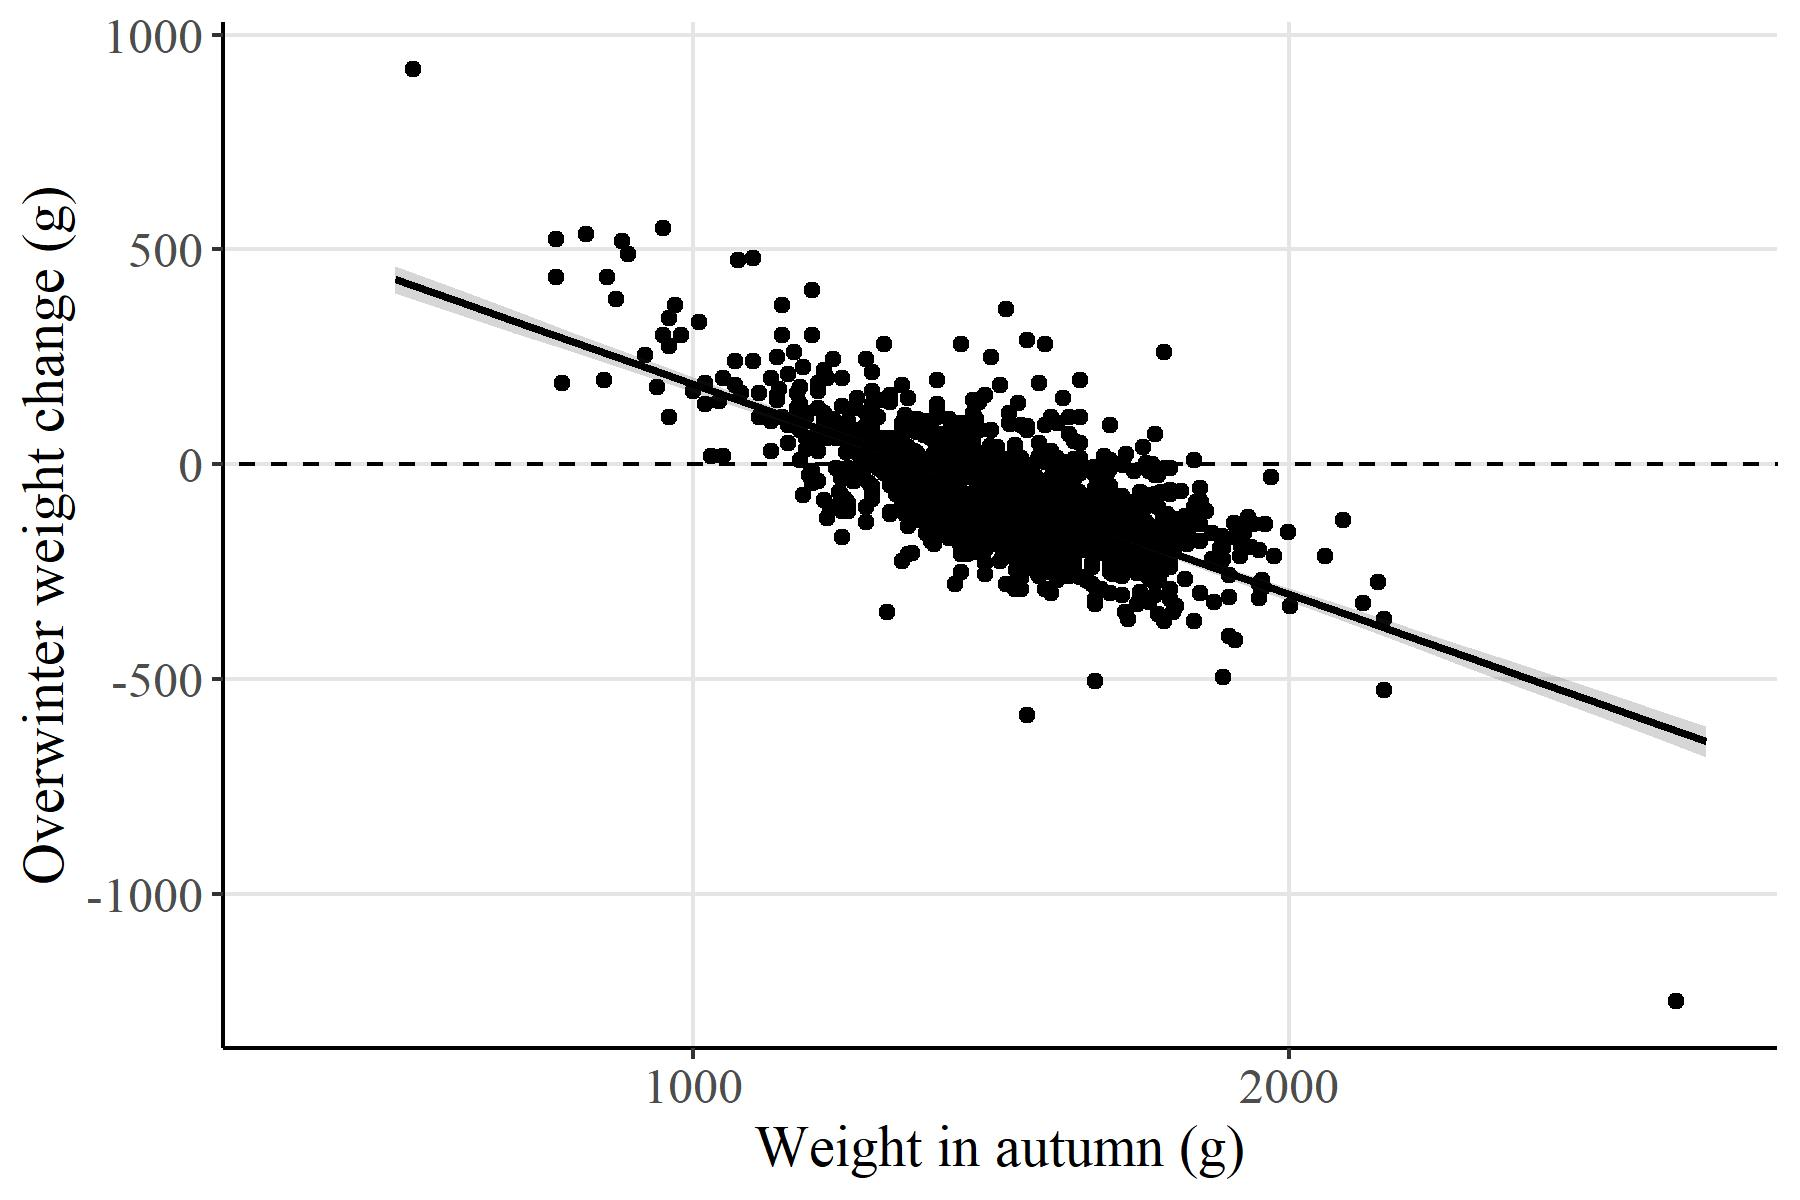
\includegraphics{Output/Figures/hodges_figure.jpeg}
\caption{Figure 2. Linear relationship between hare overwinter weight
loss in response to hare weight in the previous autumn on an individual
basis. Weight loss is the difference between body weight in autumn
(average from September -- November) and spring (average from March and
April). Line uses data from 1977 -- 2022.}
\end{figure}

\begin{figure}
\centering
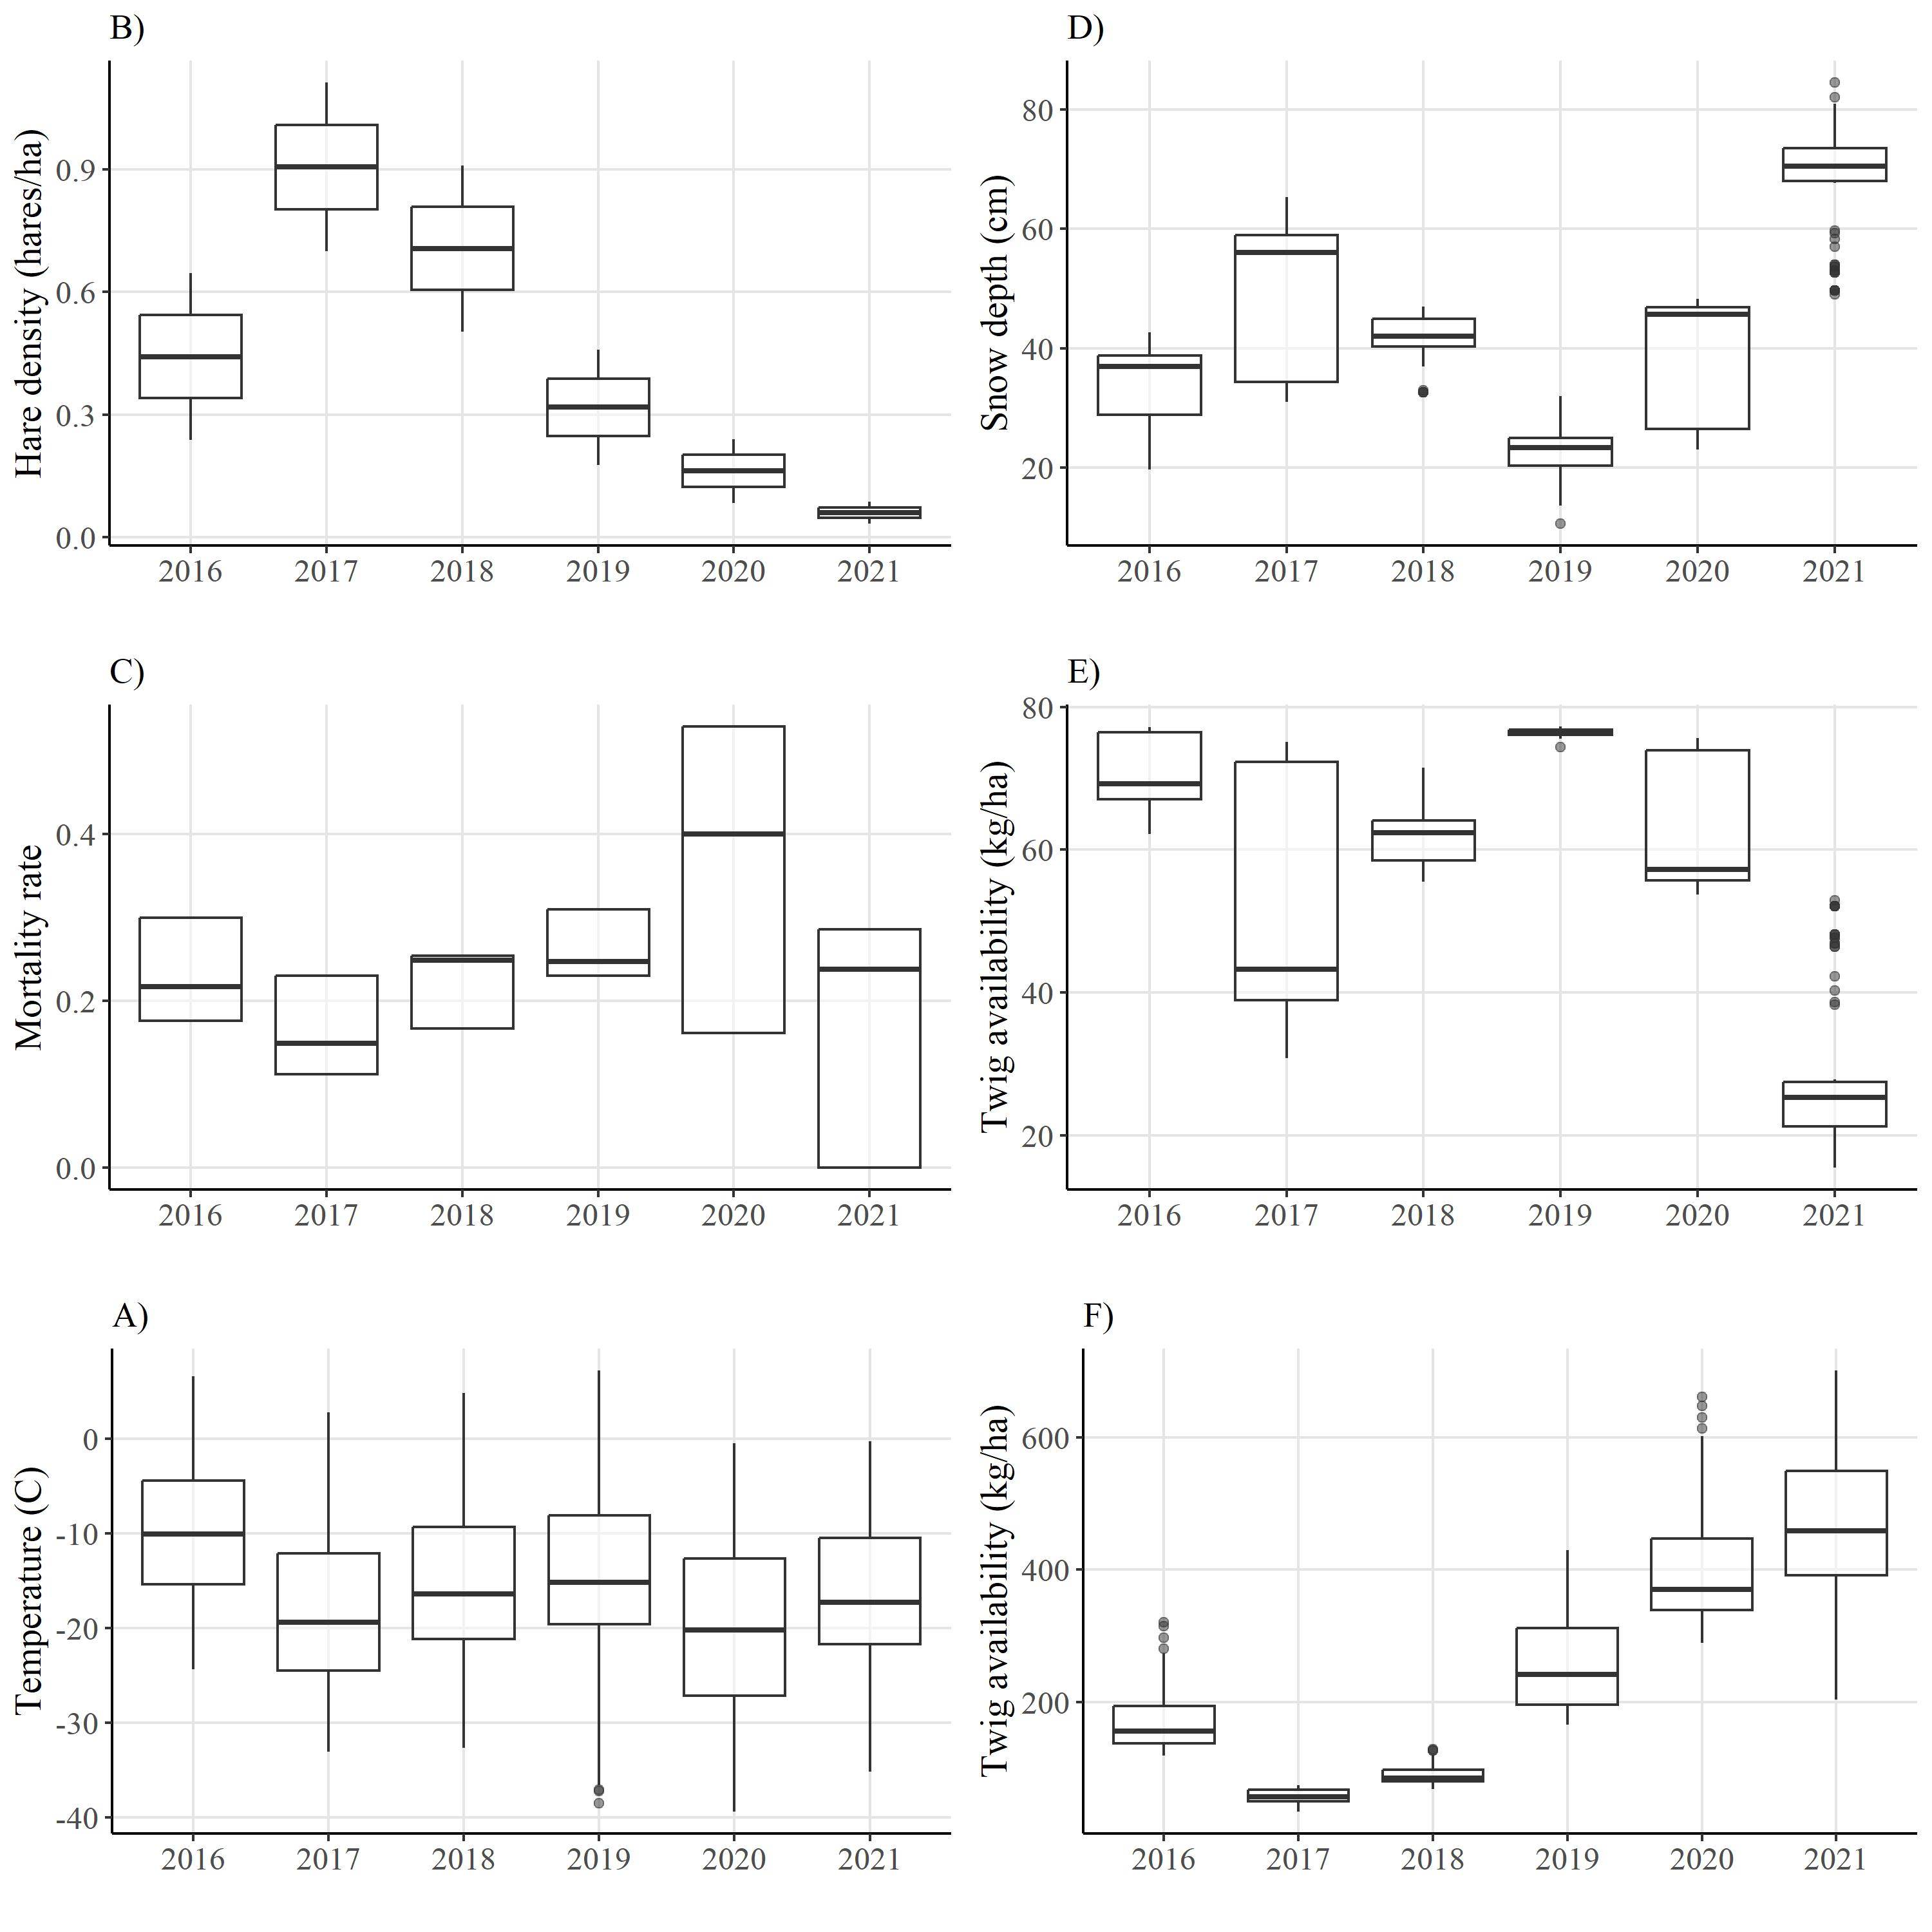
\includegraphics{Output/Figures/env_summary_figure1.jpeg}
\caption{Figure 3. Means by winter for A) daily mean temperature (C), B)
daily hare density (hares/hectare), C) monthly mortality rate, D) daily
snow depth (cm), E) daily willow twig availability (kg/hectare), and F)
daily per capita willow twig availability (kg/hare). Data includes all
values collected in January through March for each winter.}
\end{figure}

\begin{figure}
\centering
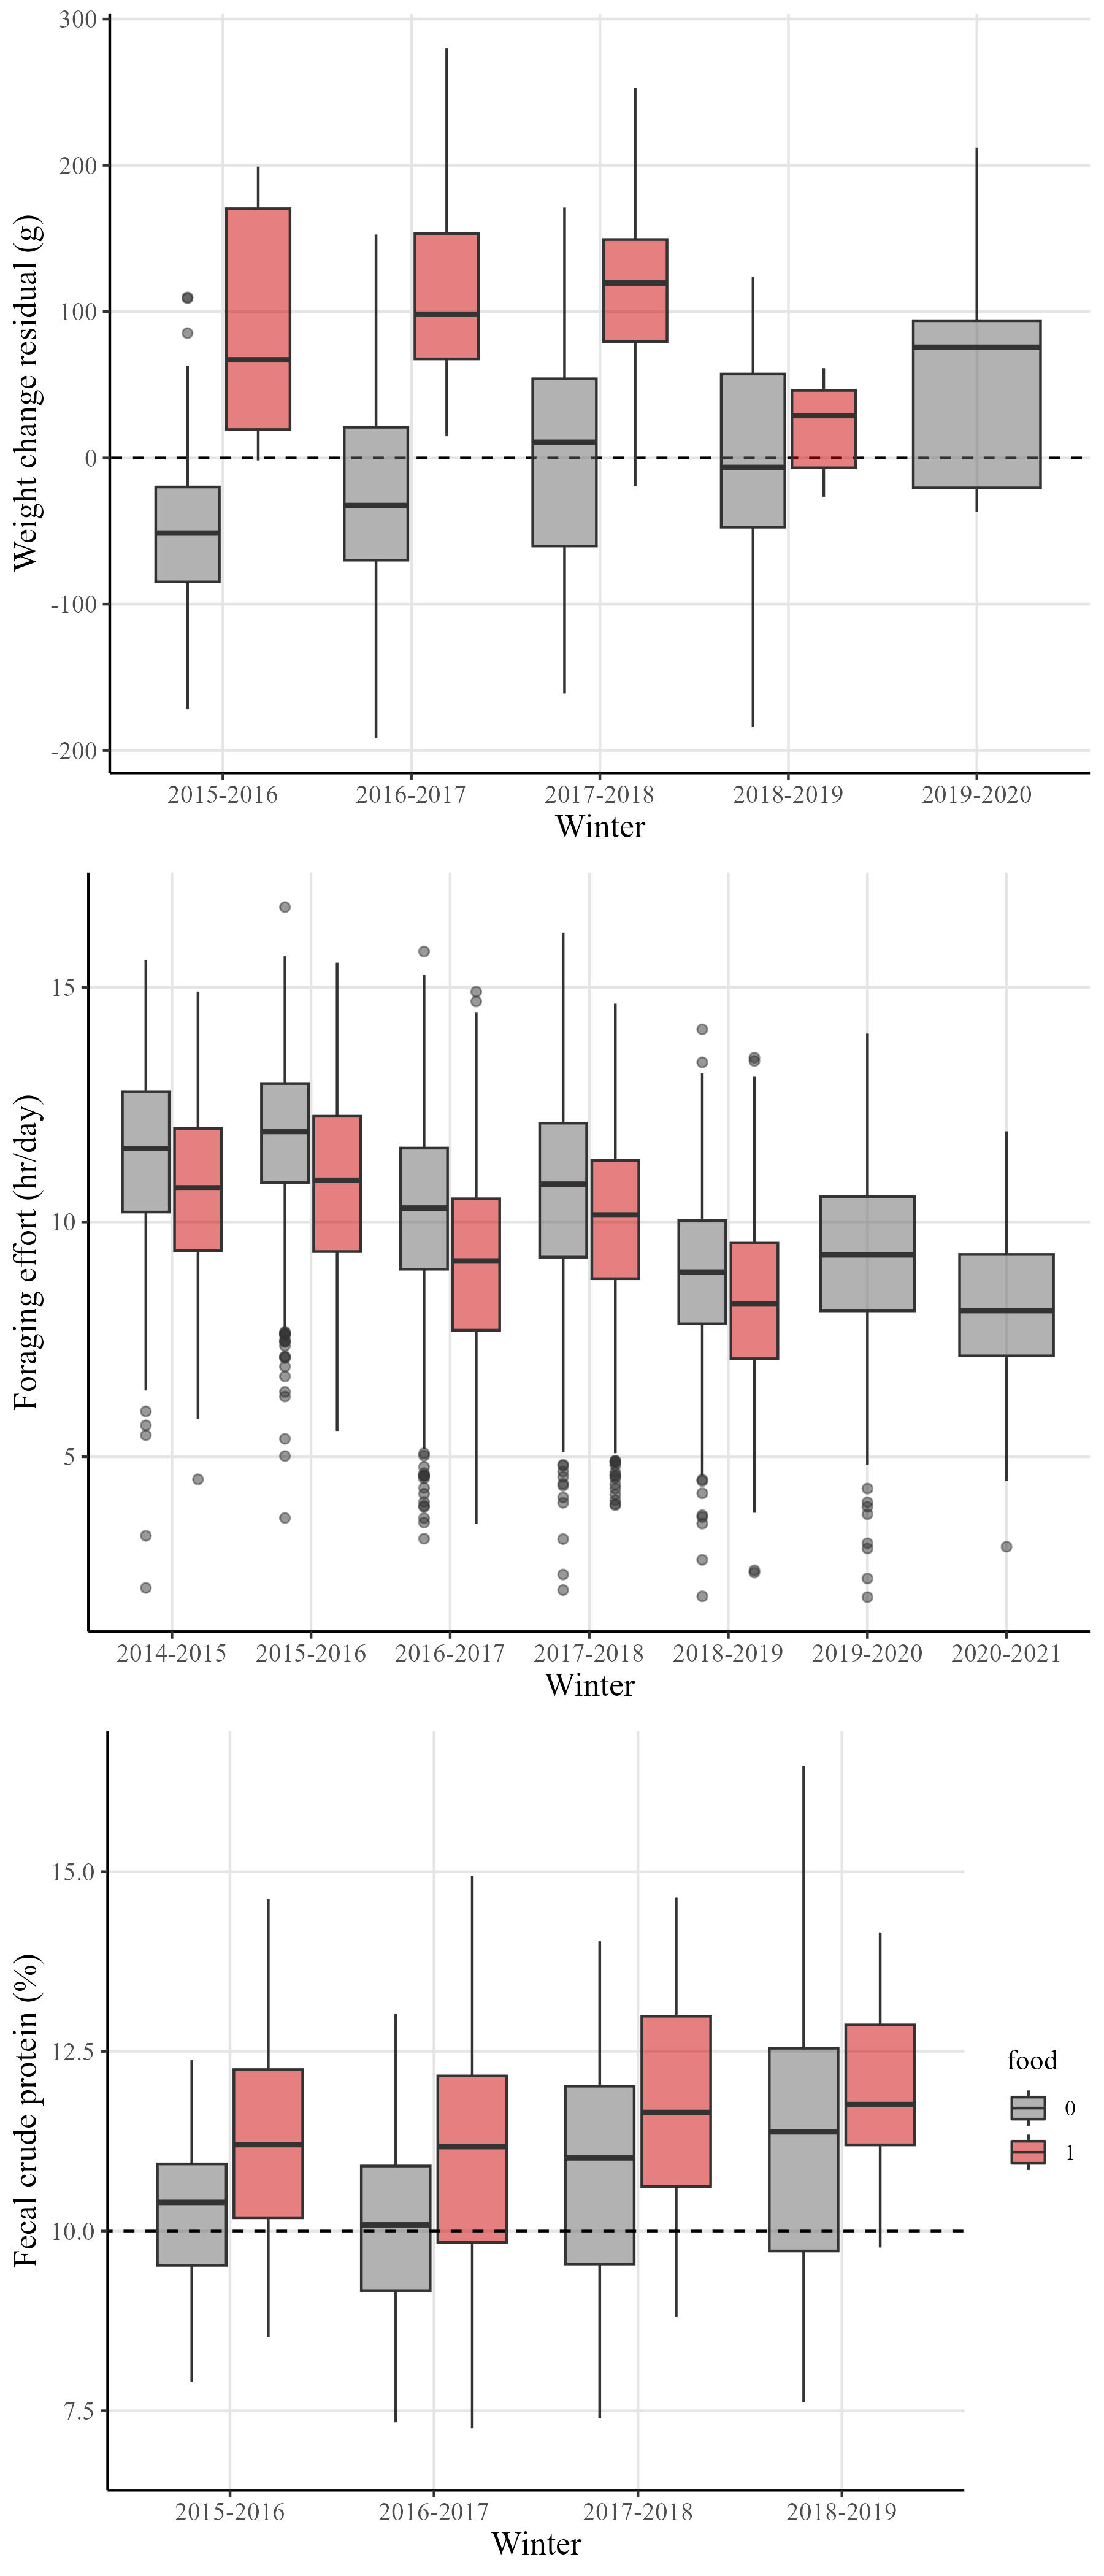
\includegraphics{Output/Figures/dep_var_figure.jpeg}
\caption{Figure 4. Mean A) overwinter weight change residuals (g), B)
fecal protein content (\%), C) and daily foraging effort (hours/day) by
winter. Boxes are colored according to food supplementation treatment
(red = food add, grey = control).}
\end{figure}

Categorizing years into high's and low's for each respective
environmental variable we get:

Snow, Temperature, and twig availability always matched. While density
and per capita always matched. Therefore, we categorized years using
density and twig availability, either high or low, to conduct a two-way
anova.

\begin{figure}
\centering
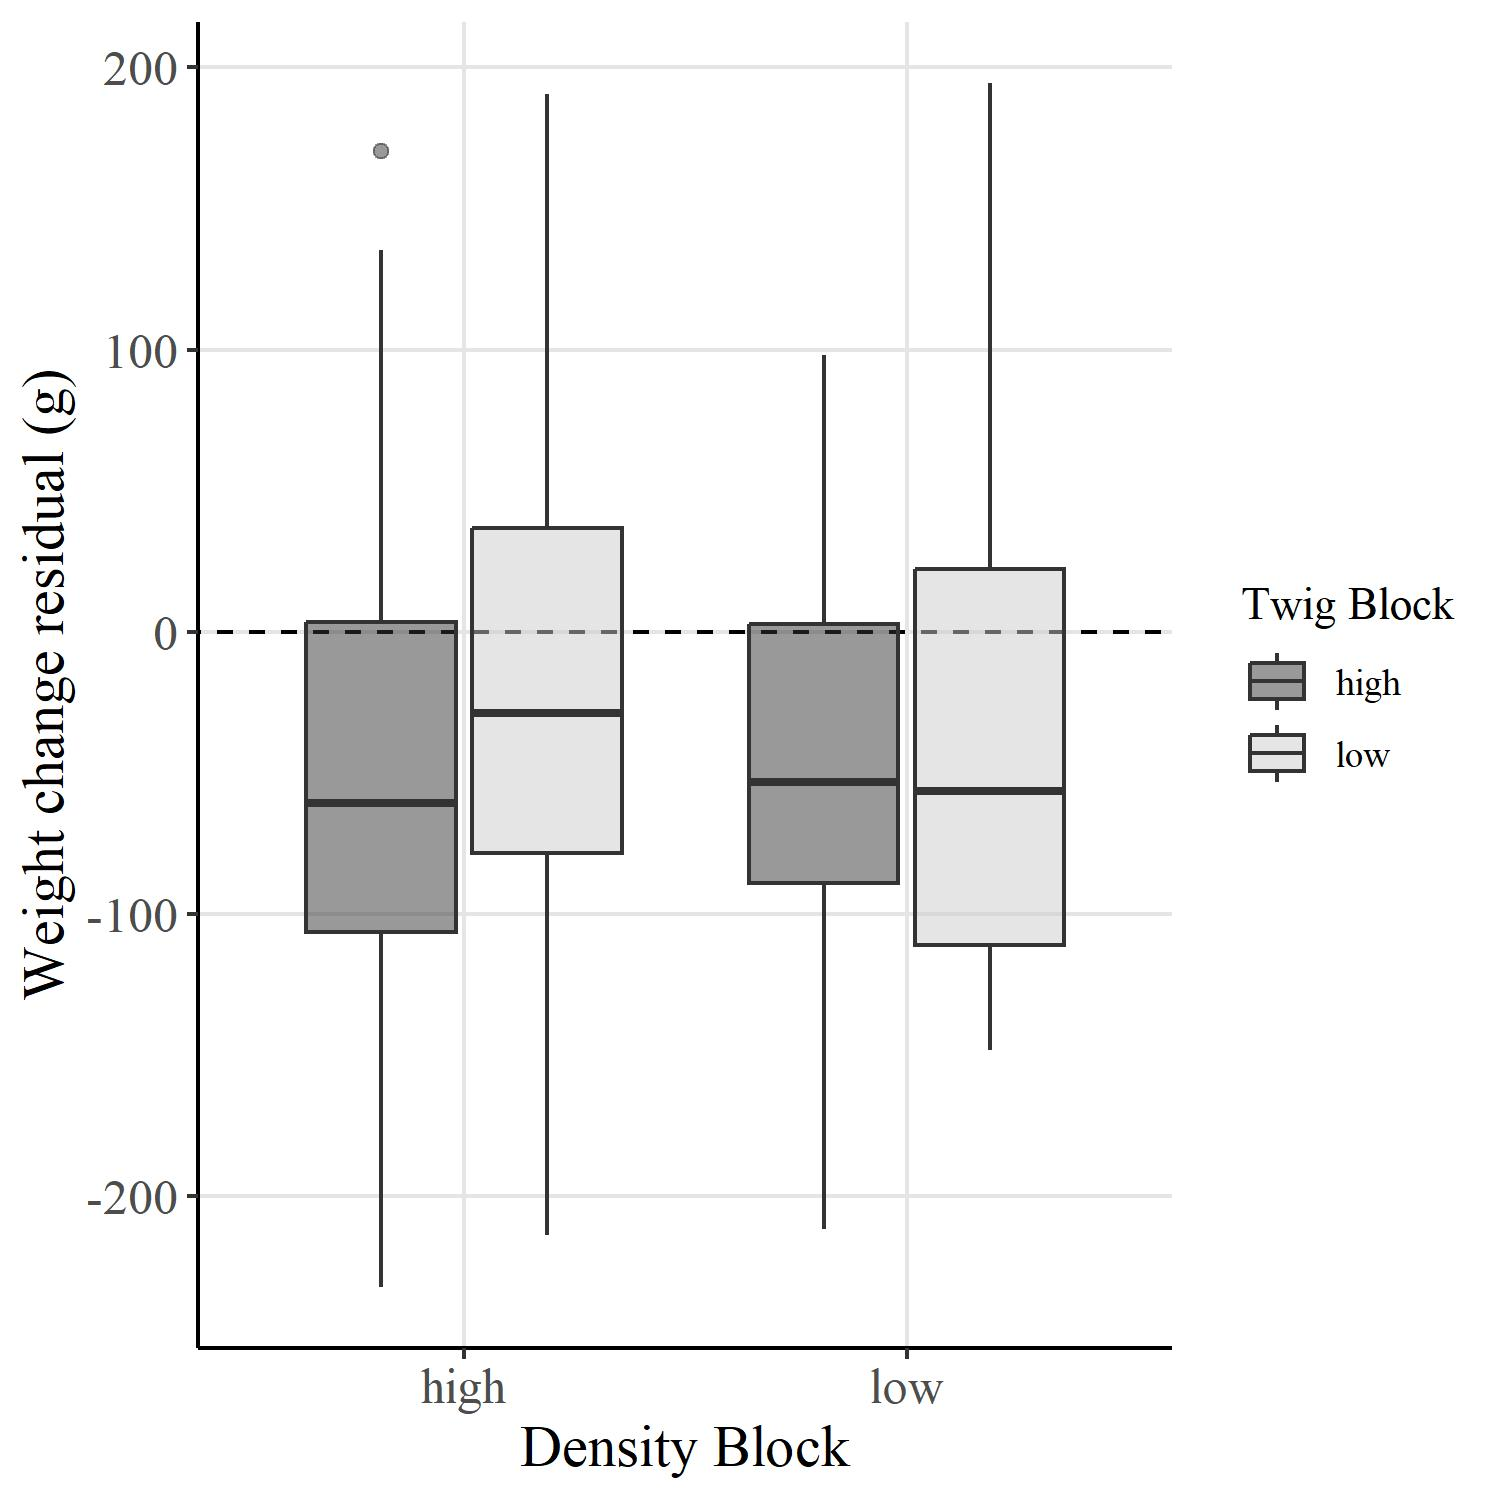
\includegraphics{Output/Figures/weight_anova.jpeg}
\caption{Figure 5. Results from the two-way anova testing how high
vs.~low hare density years and high vs.~low twig availability years
affect overwinter weight loss. Twig availability was significant.}
\end{figure}

\begin{figure}
\centering
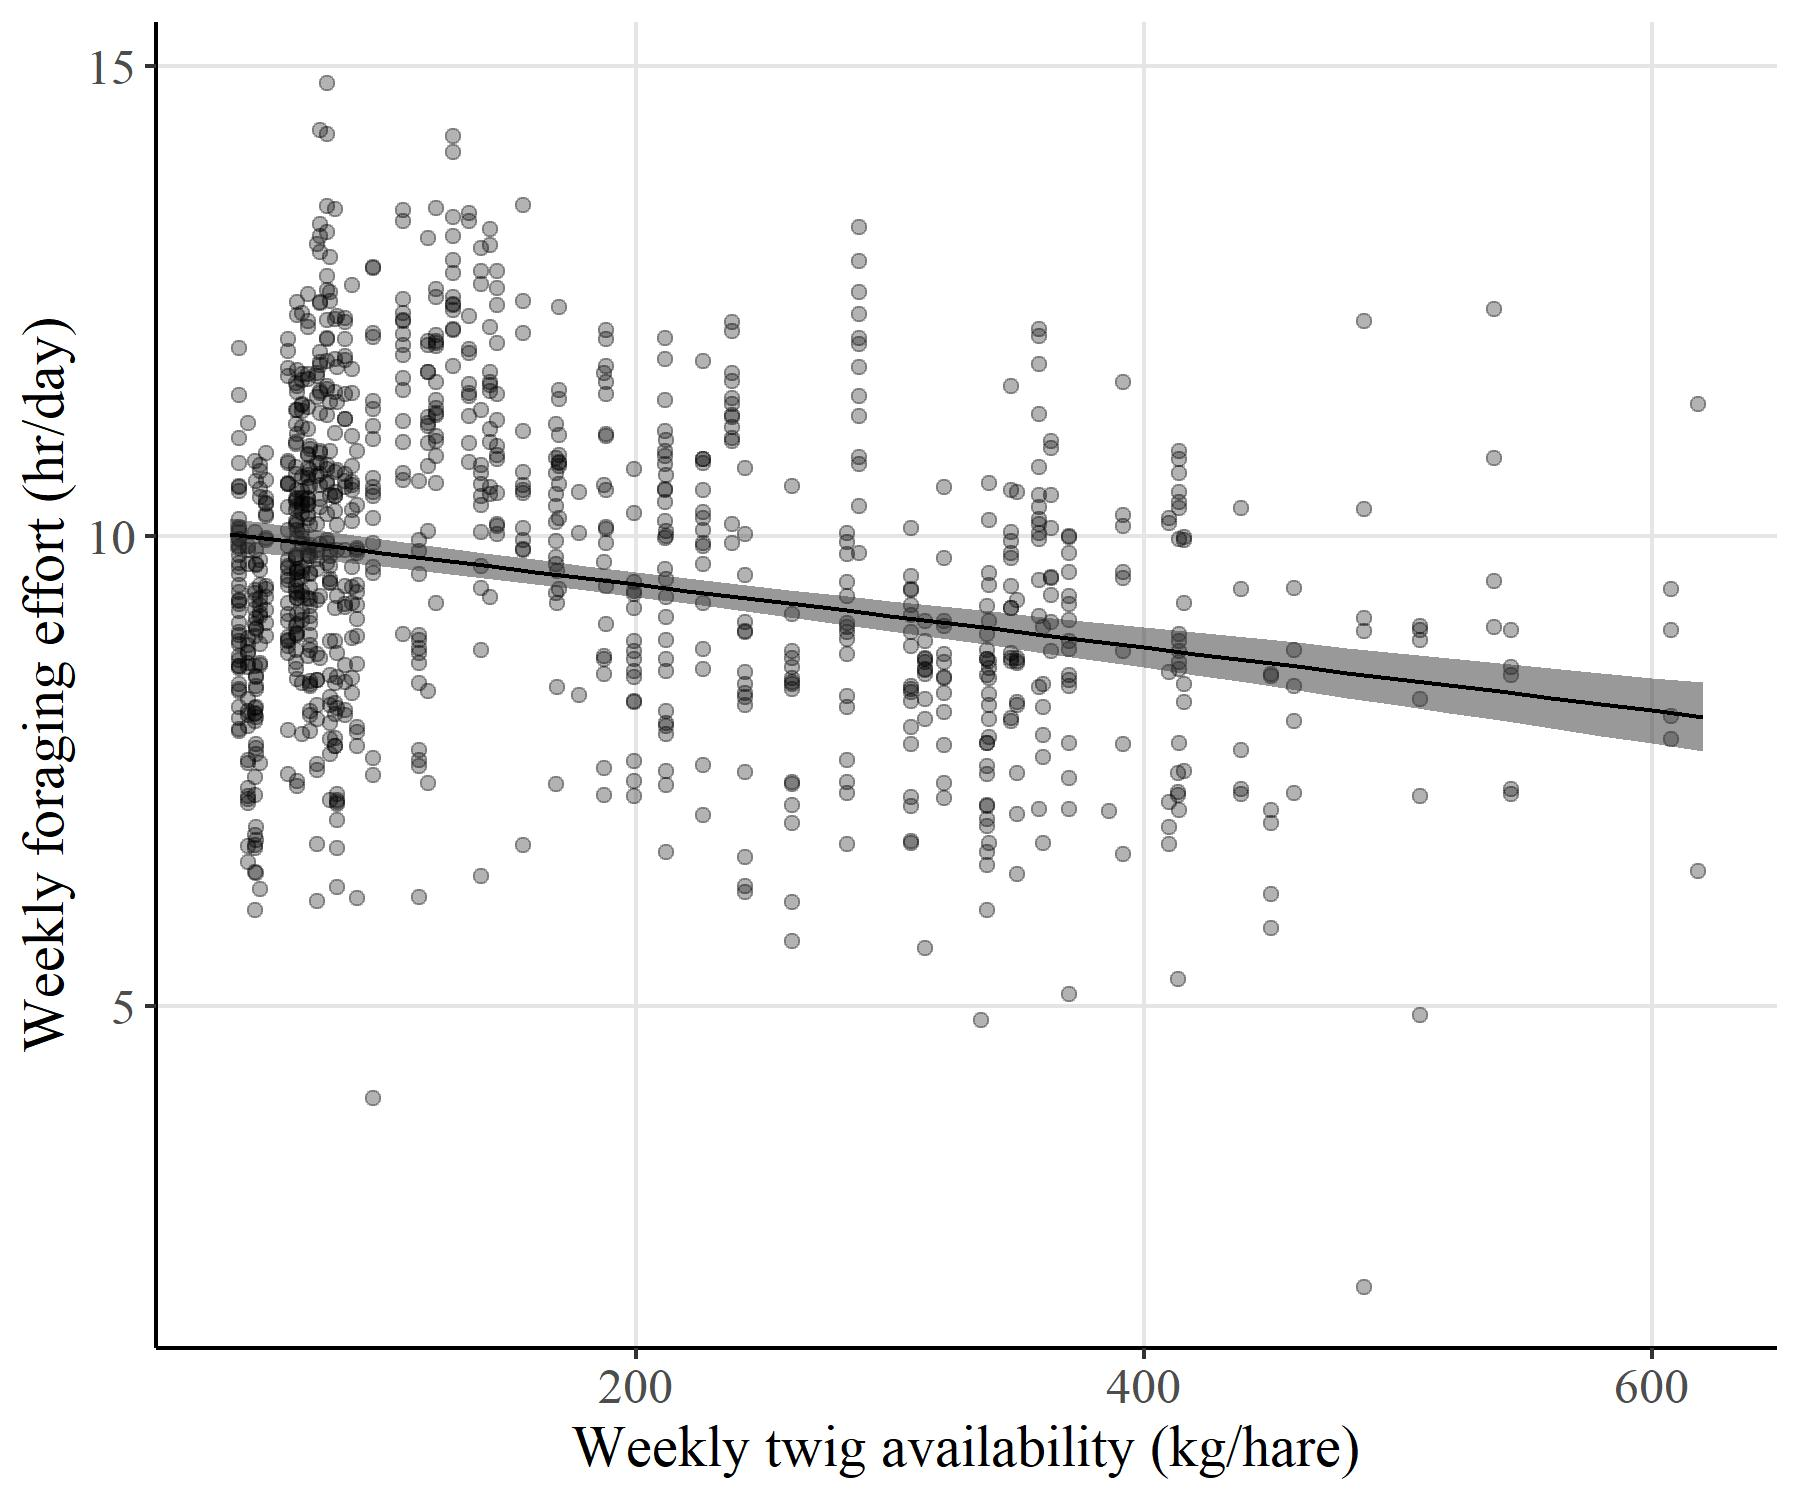
\includegraphics{Output/Figures/foraging_percap_control.jpeg}
\caption{Figure 6.}
\end{figure}

\begin{figure}
\centering
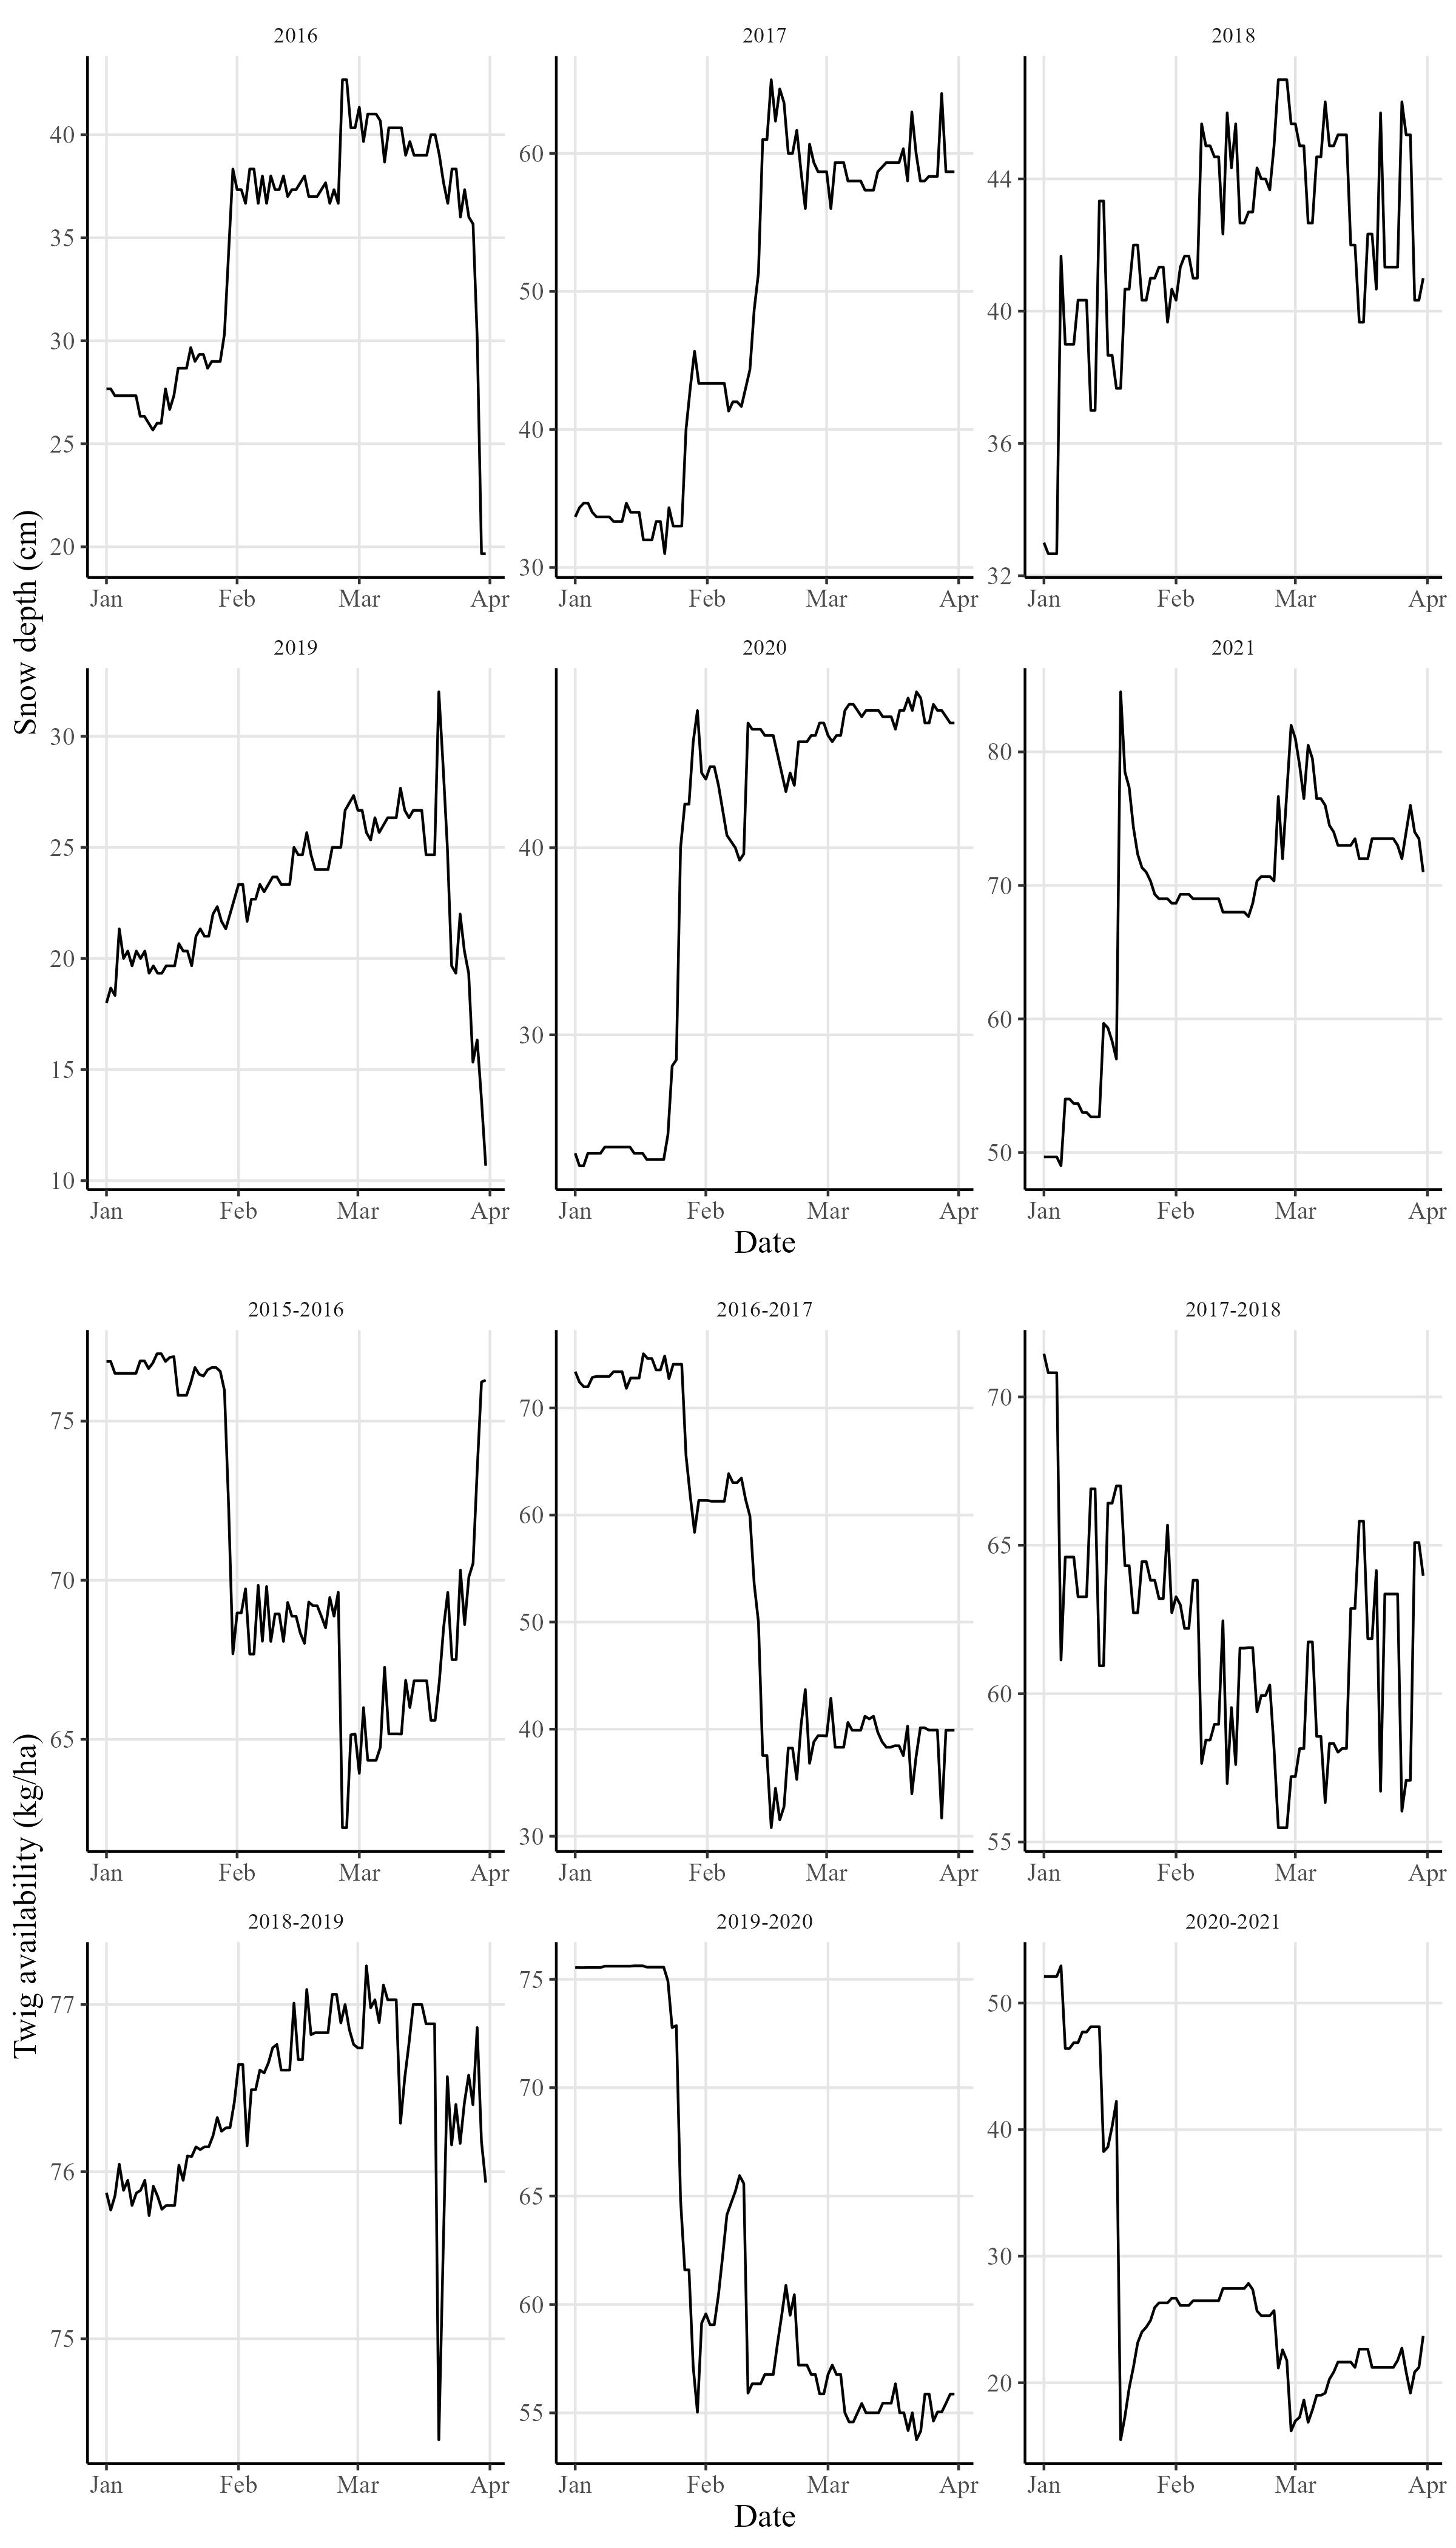
\includegraphics{Output/Figures/snow_daily_figure.jpeg}
\caption{Figure 5. Daily snow depth by winter.}
\end{figure}

\begin{figure}
\centering
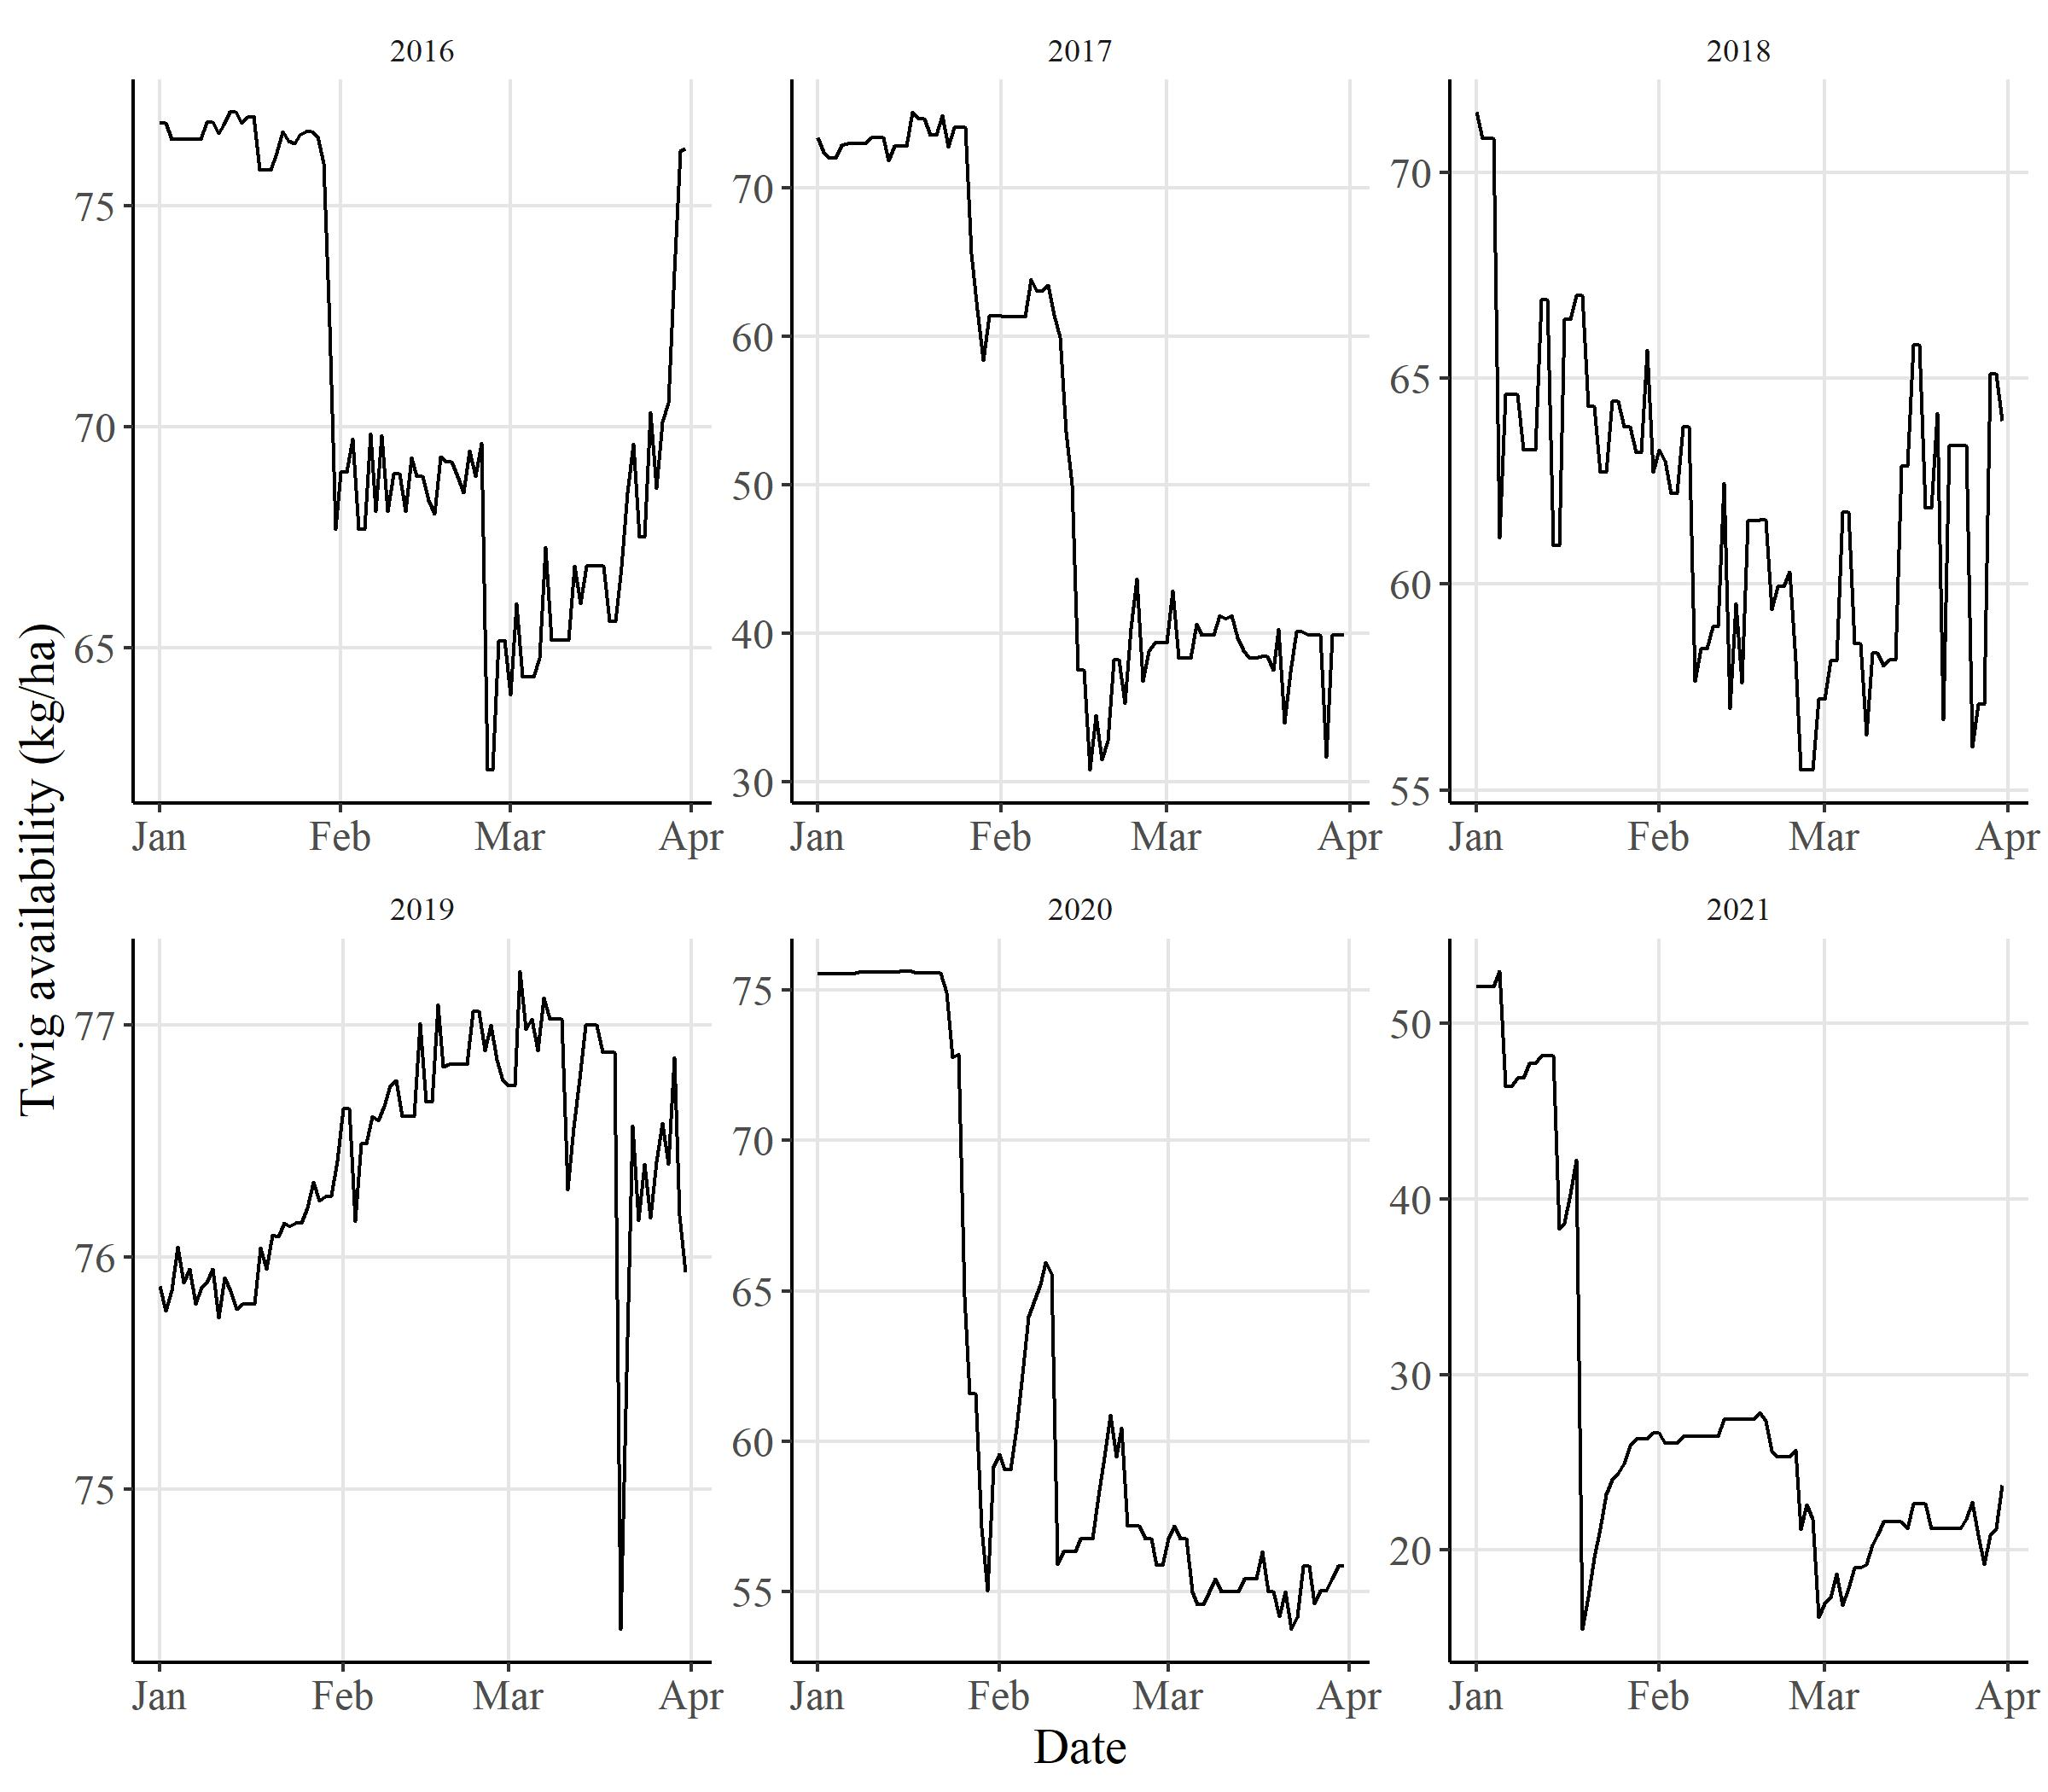
\includegraphics{Output/Figures/twig_daily_figure.jpeg}
\caption{Figure 6. Daily twig availability (kg/ha) by winter.}
\end{figure}

\begin{figure}
\centering
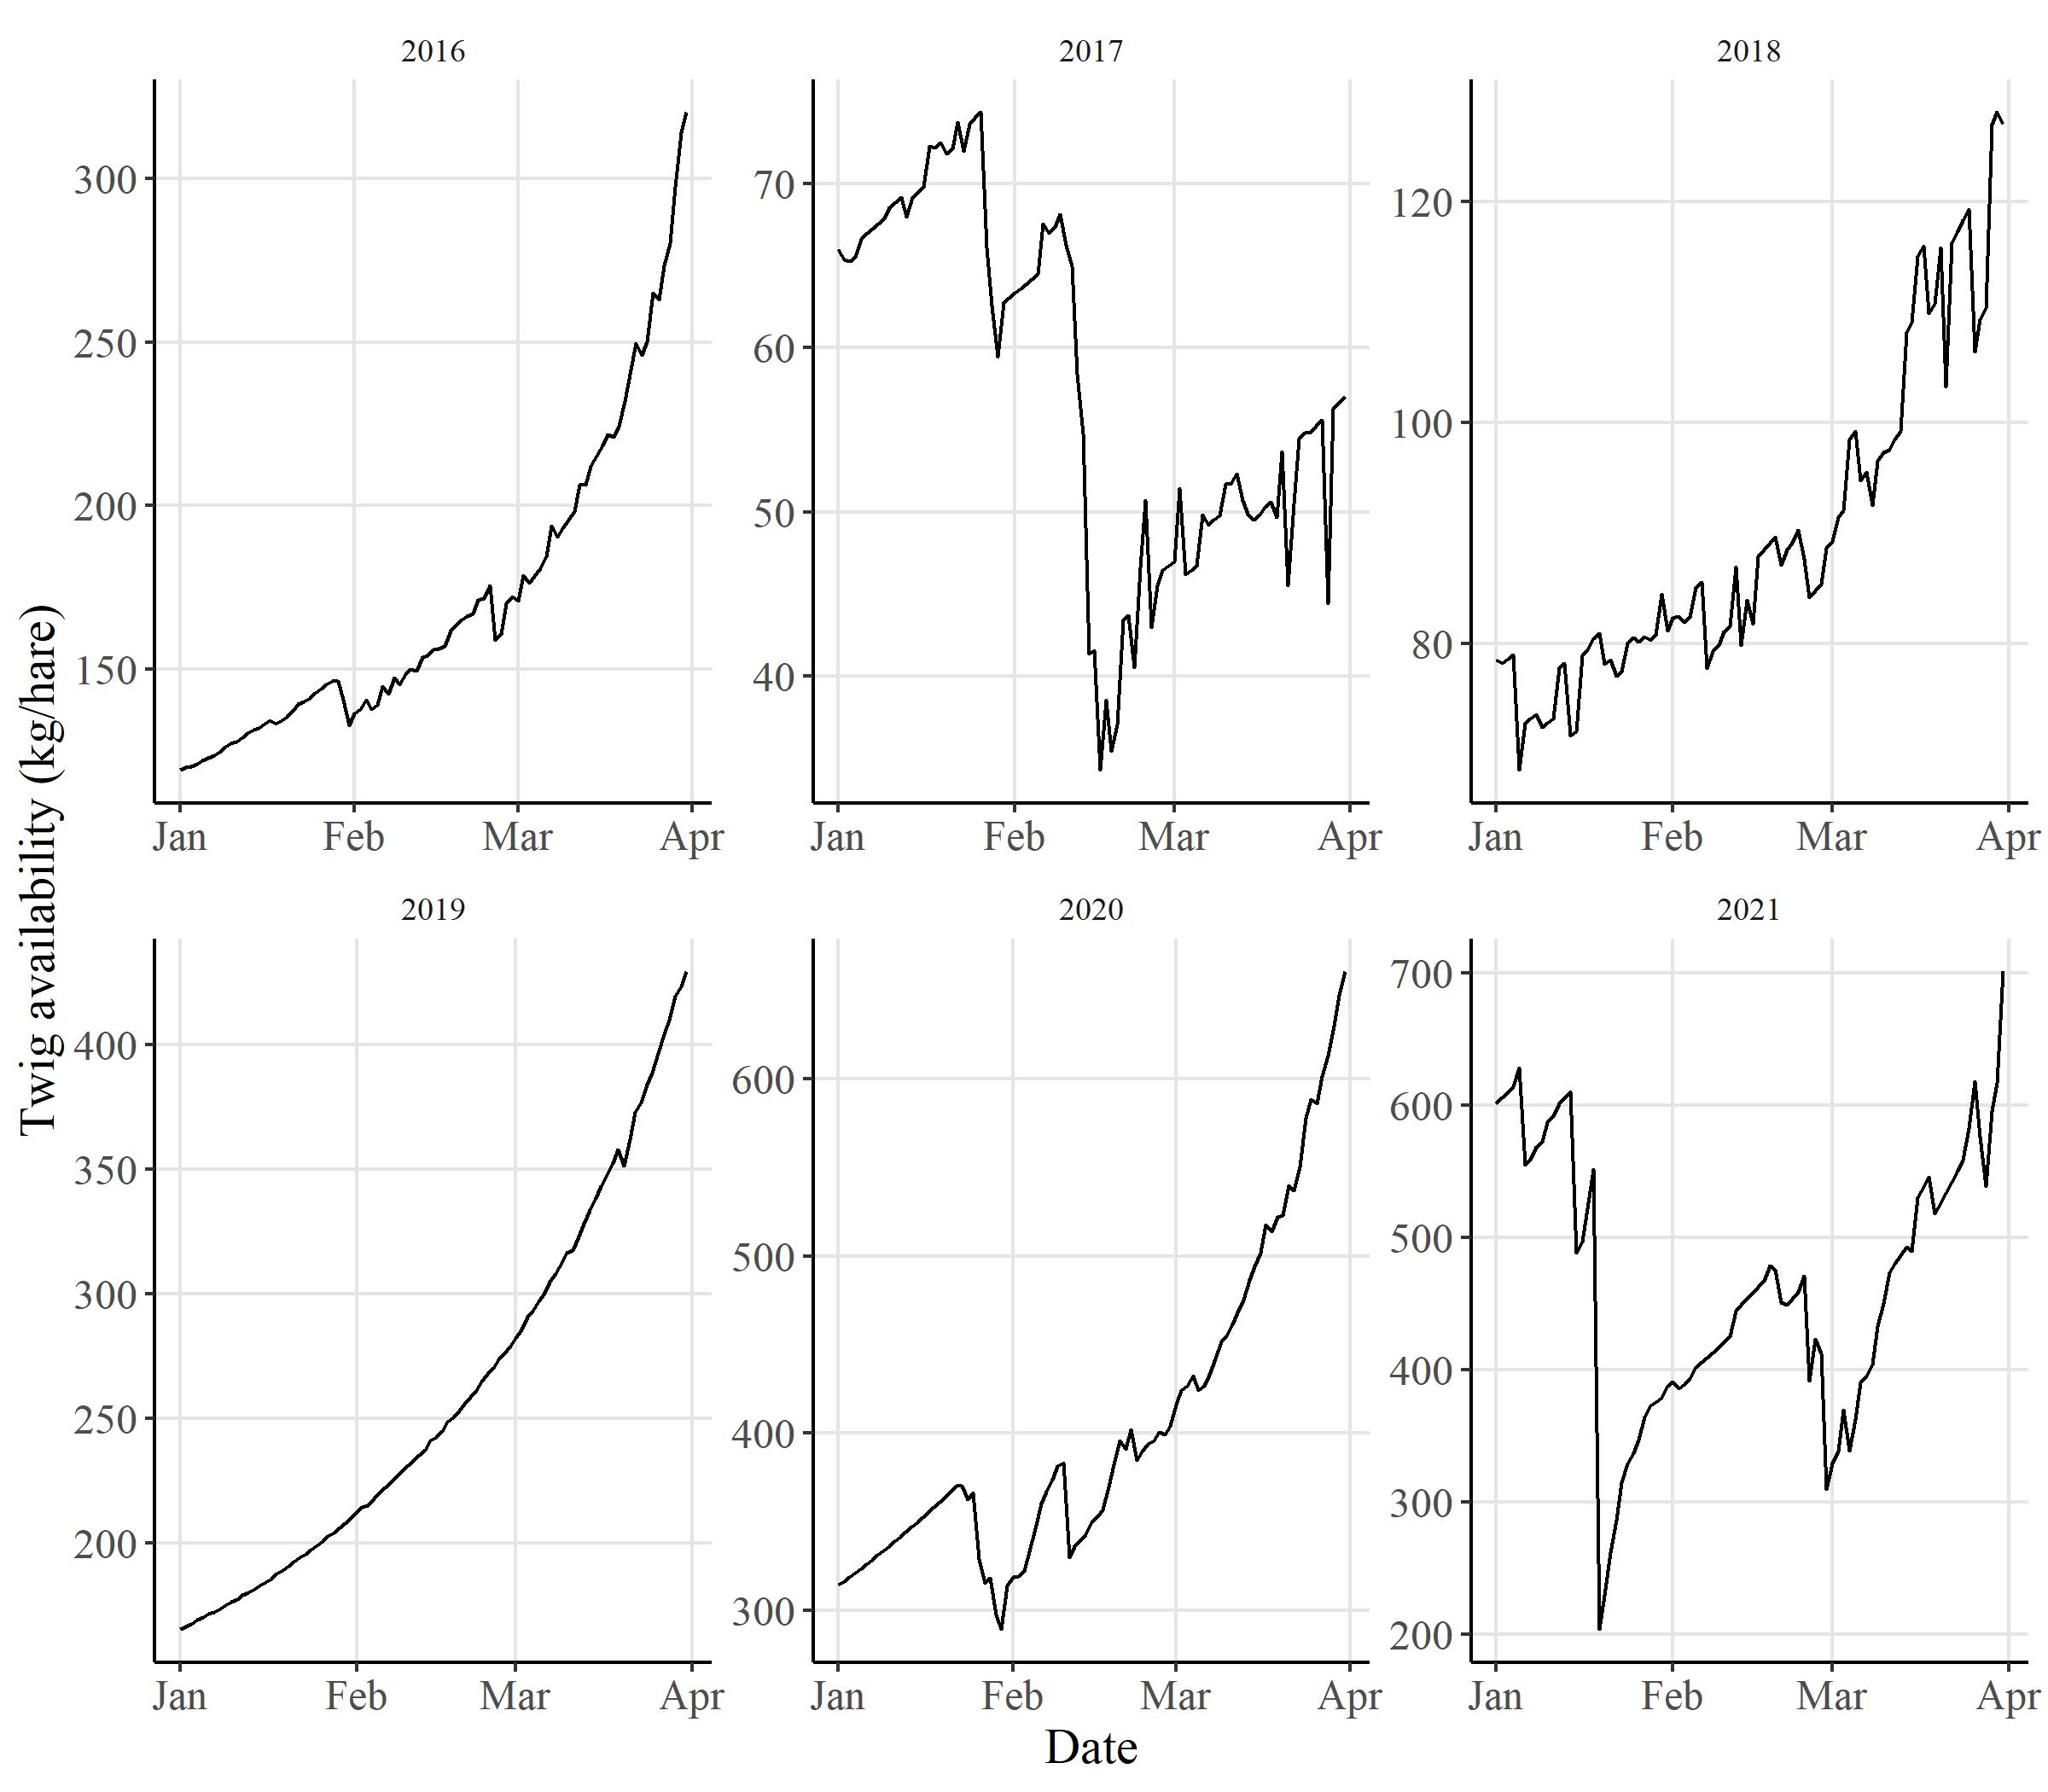
\includegraphics{Output/Figures/percap_daily_figure.jpeg}
\caption{Figure 7. Daily per capita twig (kg/hare) availability by
winter.}
\end{figure}

\end{document}
